\documentclass{nuistthesis}

% 导入包
\usepackage{xcolor}
\usepackage{enumerate}
\usepackage{url}
\usepackage{listings}

% %%%% 变量定义 %%%%
\nuistthesisset {
    title = 南京信息工程大学硕士学位论文\LaTeX 模板,
    titleen = The \LaTeX Template for Master Thesis of Nanjing University of Information Science $\&$ Technology,
    name = Alrash,
    degree = 工学硕士,
    institute = 计算机与软件学院,    
    keywordscn = 论文要求\delimitercn 样例模板,
    keywordsen = standardization of writing\delimiteren latex template,
}

\begin{document}

\includefrontmatter

\abstract {
}{
}

\includelistpage

\mainmatterstart

\chapter{学位论文部分要求}

\section{摘要}

硕士: 500~1000字(小4号宋体字,{\bfseries 限一页},含3-5个关键词),其内容同前言,但要更简明、精辟,可以独立使用,也可以引用和作为推广介绍;与中文对应的英文摘要亦含关键词。

\section{正文}

\subsection{前言/绪论}

硕士:2000—5000字左右。应包含学位论文的主要信息,包括本领域的前沿动态、作者的研究目的、研究方法、研究成果和最终结论,其重点是作者的创新性成果和结论;

\subsection{正文}

学位论文的主体,要求理科博士学位论文一般不低于4万字;理科硕士学位论文一般不低于\textcolor{red}{2}万字;

\subsection{结论}

应该观点明确、严谨、完整、准确,文字必须简明扼要,要阐明本人在科研工作中的创造性成果、新见解及其意义,本文成果在本领域中的地位和作用,对存在的问题和不足应做出客观的叙述和提出建议;

\subsection{参考文献与注释}

按文中出现的顺序列出直接引用的主要参考文献,注释可列在所在页下方。

(1)作者简介主要包括本人简历、所从事的主要研究方向和取得的科研成果,要求语句精炼,硕士生字数应控制在1000字以内,博士生字数控制在2000字以内;
(2)作者简介内容按照下列次序编排:
基本情况,包括姓名、性别、年龄、籍贯或出生地等
从大学开始的学习和工作简历(包括毕业学校、院系、专业、学习时间;工作的单位、职务和时段等);
(3)本阶段学位攻读期间课程学习情况,包括学习课程的门数、总学分数、学位课程学分数等;
(4)参加研究课题(或工程设计)情况,包括课题名称、课题类别(属国家级、省部级、横向协作、子课题属那一级课题等)、研究时段、本人承担任务及完成情况;
(5)研究生在学期间公开发表的学术论文目录和取得的其他学术成果清单(此部分单列,作为学位授予的参考条件)。学术论文包括期刊(杂志)论文和学术会议论文,其他学术成果包括学术专著、科技获奖成果、鉴定成果、专利、已完成的重要工程设计(或工程应用)项目等。该学术论文和成果清单需要经过导师认可的内容才可以列入;
按照参考文献中论文或著作的著录格式依据时间顺序排列学术著作和成果,并按顺序列出全部作者名字;
(6)学术报告和非公开发表论文情况,以及研究生非在学期间发表的学术论文目录和取得的其他学术成果等。

\section{附录}

\subsection{作者简介}

包括在学期间发表的论文和取得的学术成果清单:

\renewcommand\labelenumi{(\theenumi)}
\begin{enumerate}
    \item 作者简介主要包括本人简历、所从事的主要研究方向和取得的科研成果,要求语句精炼,硕士生字数应控制在1000字以内
    \item 作者简介内容按照下列次序编排:
    \begin{itemize}
        \item 基本情况,包括姓名、性别、年龄、籍贯或出生地等
        \item 从大学开始的学习和工作简历(包括毕业学校、院系、专业、学习时间;工作的单位、职务和时段等)
    \end{itemize}
   \item 本阶段学位攻读期间课程学习情况,包括学习课程的门数、总学分数、学位课程学分数等
   \item 参加研究课题(或工程设计)情况,包括课题名称、课题类别(属国家级、省部级、横向协作、子课题属那一级课题等)、研究时段、本人承担任务及完成情况
   \item 学术报告和非公开发表论文情况,以及研究生非在学期间发表的学术论文目录和取得的其他学术成果等
\end{enumerate}


\subsection{成果清单}

研究生在学期间公开发表的学术论文目录和取得的其他学术成果清单(此部分单列,作为学位授予的参考条件)。学术论文包括期刊(杂志)论文和学术会议论文,其他学术成果包括学术专著、科技获奖成果、鉴定成果、专利、已完成的重要工程设计(或工程应用)项目等。该学术论文和成果清单需要经过导师认可的内容才可以列入;
按照参考文献中论文或著作的著录格式依据时间顺序排列学术著作和成果,并按顺序列出全部作者名字;


\chapter{使用说明}

本模板在CTEX-Book的基础之上进行一定程度的排版,大部分格式为本人凭借《南京信息工程大学\hspace{1em}2019年学位论文格式及盲审格式》\cite{NUIST_thesis}及\textcolor{red}{\bfseries 个人感觉}进行排版,{\bfseries 可能}无法满足部分审核老师的需求,请注意。

同时,本模板{\bfseries 仅在XeLaTex下测试},\textcolor{red}{不能保证LuaLaTex排版},请注意。

\section{封面说明}

格式文件中,封面题目使用“华文中宋”字体,也就是需要'STZhongsong.ttf'字体文件。此文件windows自带,macOS未知,linux不存在。本模板不提供此字体下载链接,需自行下载安装,或下载后放至与nuistthesis.cls同级目录。也可使用以下命令获取:

\lstset{
    basicstyle = \small\ttfamily,
    language = bash,
    commentstyle=\color{white} \bf,
    backgroundcolor=\color{cyan},
}
\begin{lstlisting}
git reset --hard HEAD^
\end{lstlisting}


\section{全局变量}

本模板存在一个全局变量 \textbackslash nuistthesisset,其存在以下几个键值用于生成封面等信息。
\lstset{
    basicstyle = \small\ttfamily,
    language = [LaTeX]{TeX},
    commentstyle=\color{white} \bf,
    backgroundcolor=\color{cyan},
}
\begin{lstlisting}
\nuistthesisset {
    title = 中文题目,
    titleen = 英文题目,
    name = 姓名,
    mentor = 你的导师,
    comentor = 合作导师,                       % 使用\comentor显示
    degree = 学位,                             % 盲审使用 
    major = 专业名称,
    research = 研究方向,
    institute= 学院名称,
    number = 00000000000,                      % 学号
    year = 2020,
    umonth = 1,                                % 封面底部时间
    month = 1,                                 % 盲审完成时间
    day = 29,                                  % 盲审完成时间
    keywordscn = 关键词(可用\delimitercn分割,注意误空格),
    keywordsen = keywords (可用\delimiteren分割,注意误空格),
}
\end{lstlisting}

\section{额外的命令}

\subsection{命令列表}

表\ref{tab:providecommand}显示了本模板所有提供的额外命令:

\begin{table}[htbp!]
\centering
\ftfonts
\caption{提供命令列表} \label{tab:providecommand}
    \begin{tabular}{c l | c l}
        \hline
        名称 & 作用 & 名称 & 作用\\
        \hline
        includefrontmatter & 生成封面及声明页 & abstract[2] & 接受中文与英文摘要,生成对应页 \\
        includelistpage & 生成目录部分 & mainmatterstart & 声明正文开始 \\
        delimitercn & 中文关键词分隔符 & delimiteren & 英文关键词分隔符 \\
        charspace & 提供一个中文字符的空格 & ftfonts & 修正表格内容字体、大小等 \\
        material & 章节成果展示区域 & addreferencetoctl & 将参考文献加入目录\\
        comentor & 封面显示合作导师 & printer & 为双面打印预留空白页 \\
        blindtrial & 显示盲审封面(注意封面内容)\\
        \hline
    \end{tabular}
\end{table}

其中,abstract[2]表示接受两个参数;material必选一个参数,可选两个参数;其余,均无参数传递。

\subsection{abstract}

建议以下形式使用:

\lstset{
    basicstyle = \small\ttfamily,
    language = [LaTeX]{TeX},
    commentstyle=\color{white} \bf,
    backgroundcolor=\color{cyan},
}
\begin{lstlisting}
\abstract{
% 中文摘要内容
}{
% 英文摘要内容
}
\end{lstlisting}


\subsection{material}

建议以下形式使用:

\lstset{
    basicstyle = \small\ttfamily,
    language = [LaTeX]{TeX},
    commentstyle=\color{white} \bf,
    backgroundcolor=\color{cyan},
}
\begin{lstlisting}
% vspace 表示与正文间隔,默认1em
% title  表示显示文字,默认“本章部分内容出自以下论文”
\begin{material}[vspace = 1em, title = 本章部分内容出自以下论文]
    % 内容
\end{material}
\end{lstlisting}

\section{排版布局}

推荐以下排版布局:

\lstset{
    basicstyle = \small\ttfamily,
    language = [LaTeX]{TeX},
    commentstyle=\color{white} \bf,
    backgroundcolor=\color{cyan},
}
\begin{lstlisting}
\documentclass{nuistthesis}

\nuistthesisset{}               % 全局变量赋值

\begin{document}

\includefrontmatter
\abstract{}{}
\includelistpage

% 正文
\mainmatterstart

\chapter{}
\section{}
\subsection{}

\chapter{}
\section{}
\subsection{}

% 参考文献
\bibliographystyle{nuistbib}
\bibliography{sample}
\addreferencetoctl                % 参考文献追加至目录,一定放在这里

% 附录区
\appendix
\chapter{}

% 附件区
\backmatter
\chapter{致\quad{}谢}
\chapter{学生简介}

\end{document}

\end{lstlisting}

\section{合作导师及盲审封面}

本示例使用的是最终提交论文的封面,且不显示合作导师。接下来,图\ref{fig:title}内子图展示“显示合作导师、“盲审封面”的情况。

\begin{figure}[htbp!]
    \subfigure[使用\textbackslash comentor]{
        \begin{minipage}[t]{0.5 \linewidth}
            \centering
            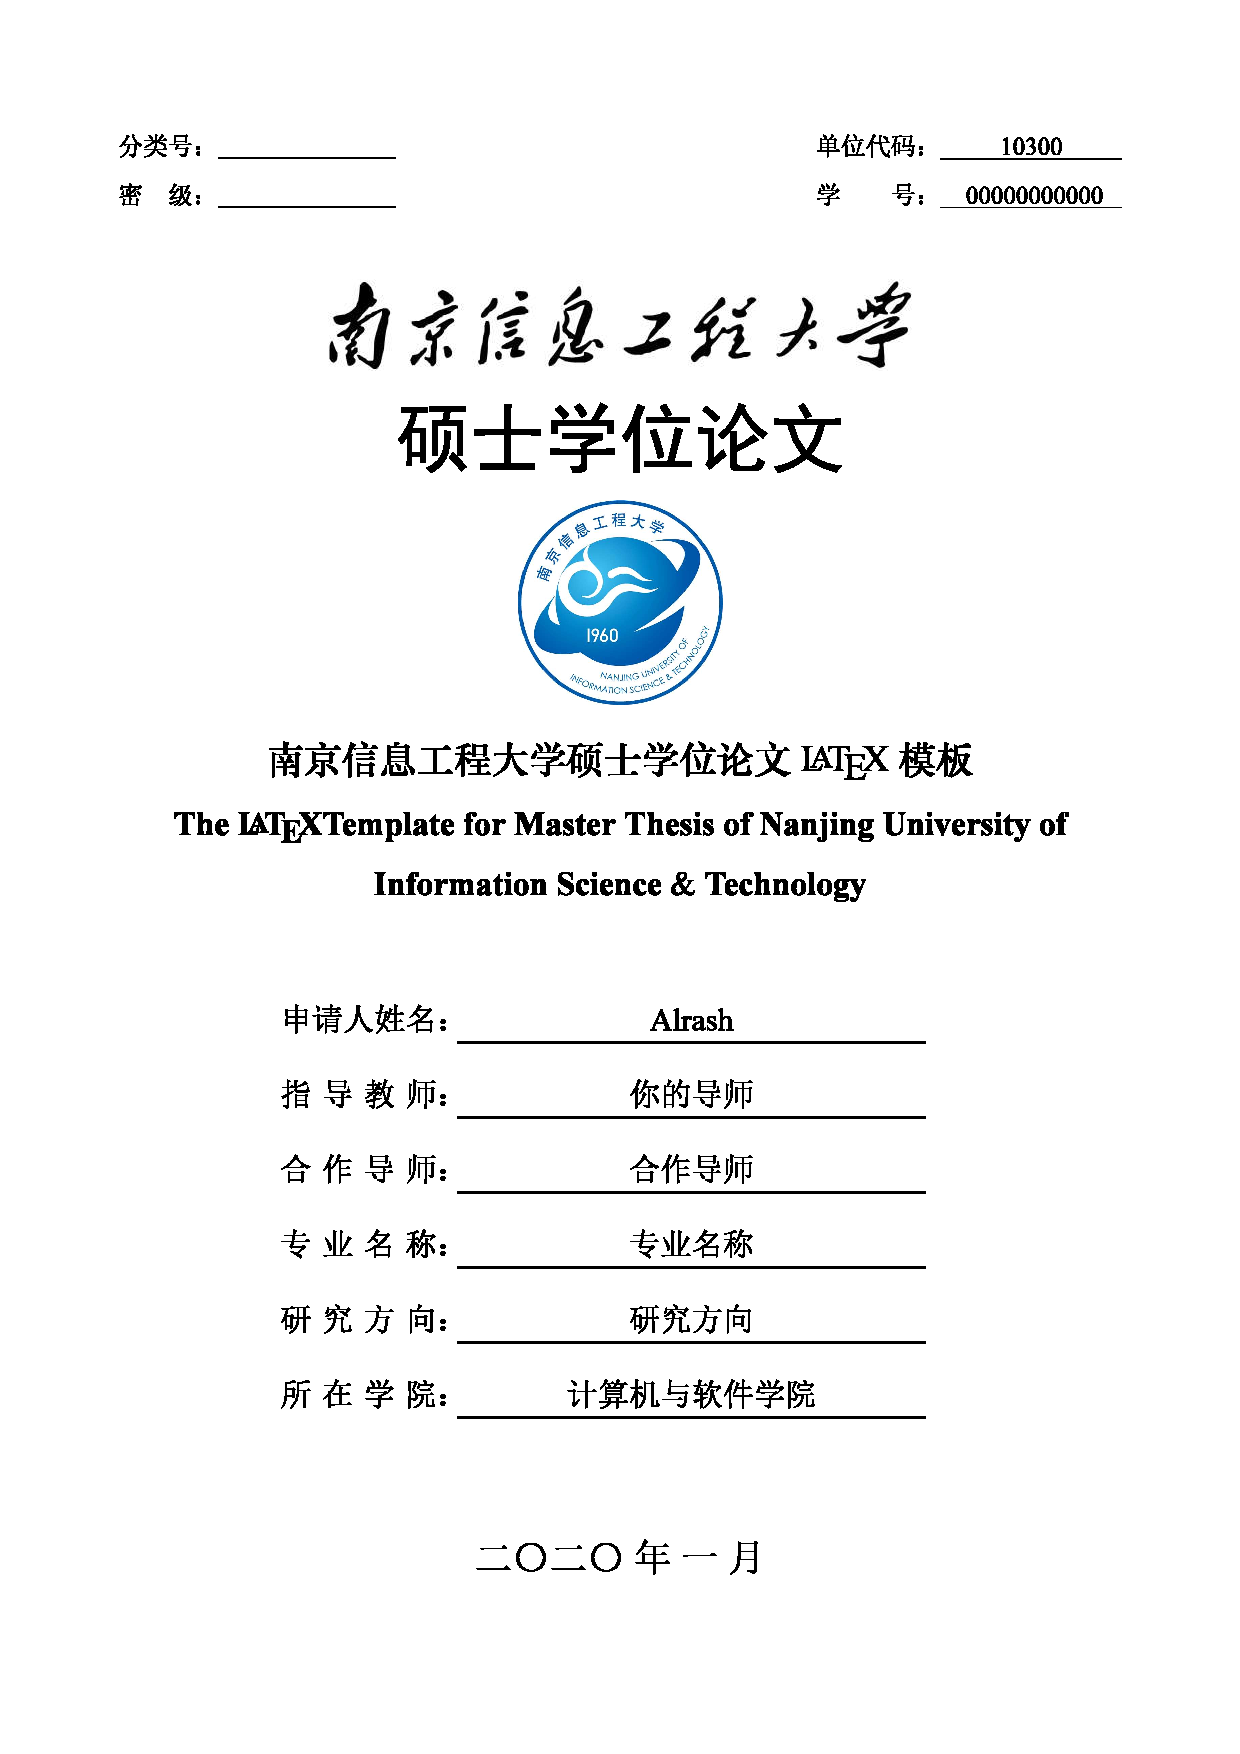
\includegraphics[width = 1\linewidth, keepaspectratio]{figs/comentor}
        \end{minipage}
    }
    \subfigure[使用\textbackslash blindtrial]{
        \begin{minipage}[t]{0.5 \linewidth}
            \centering
            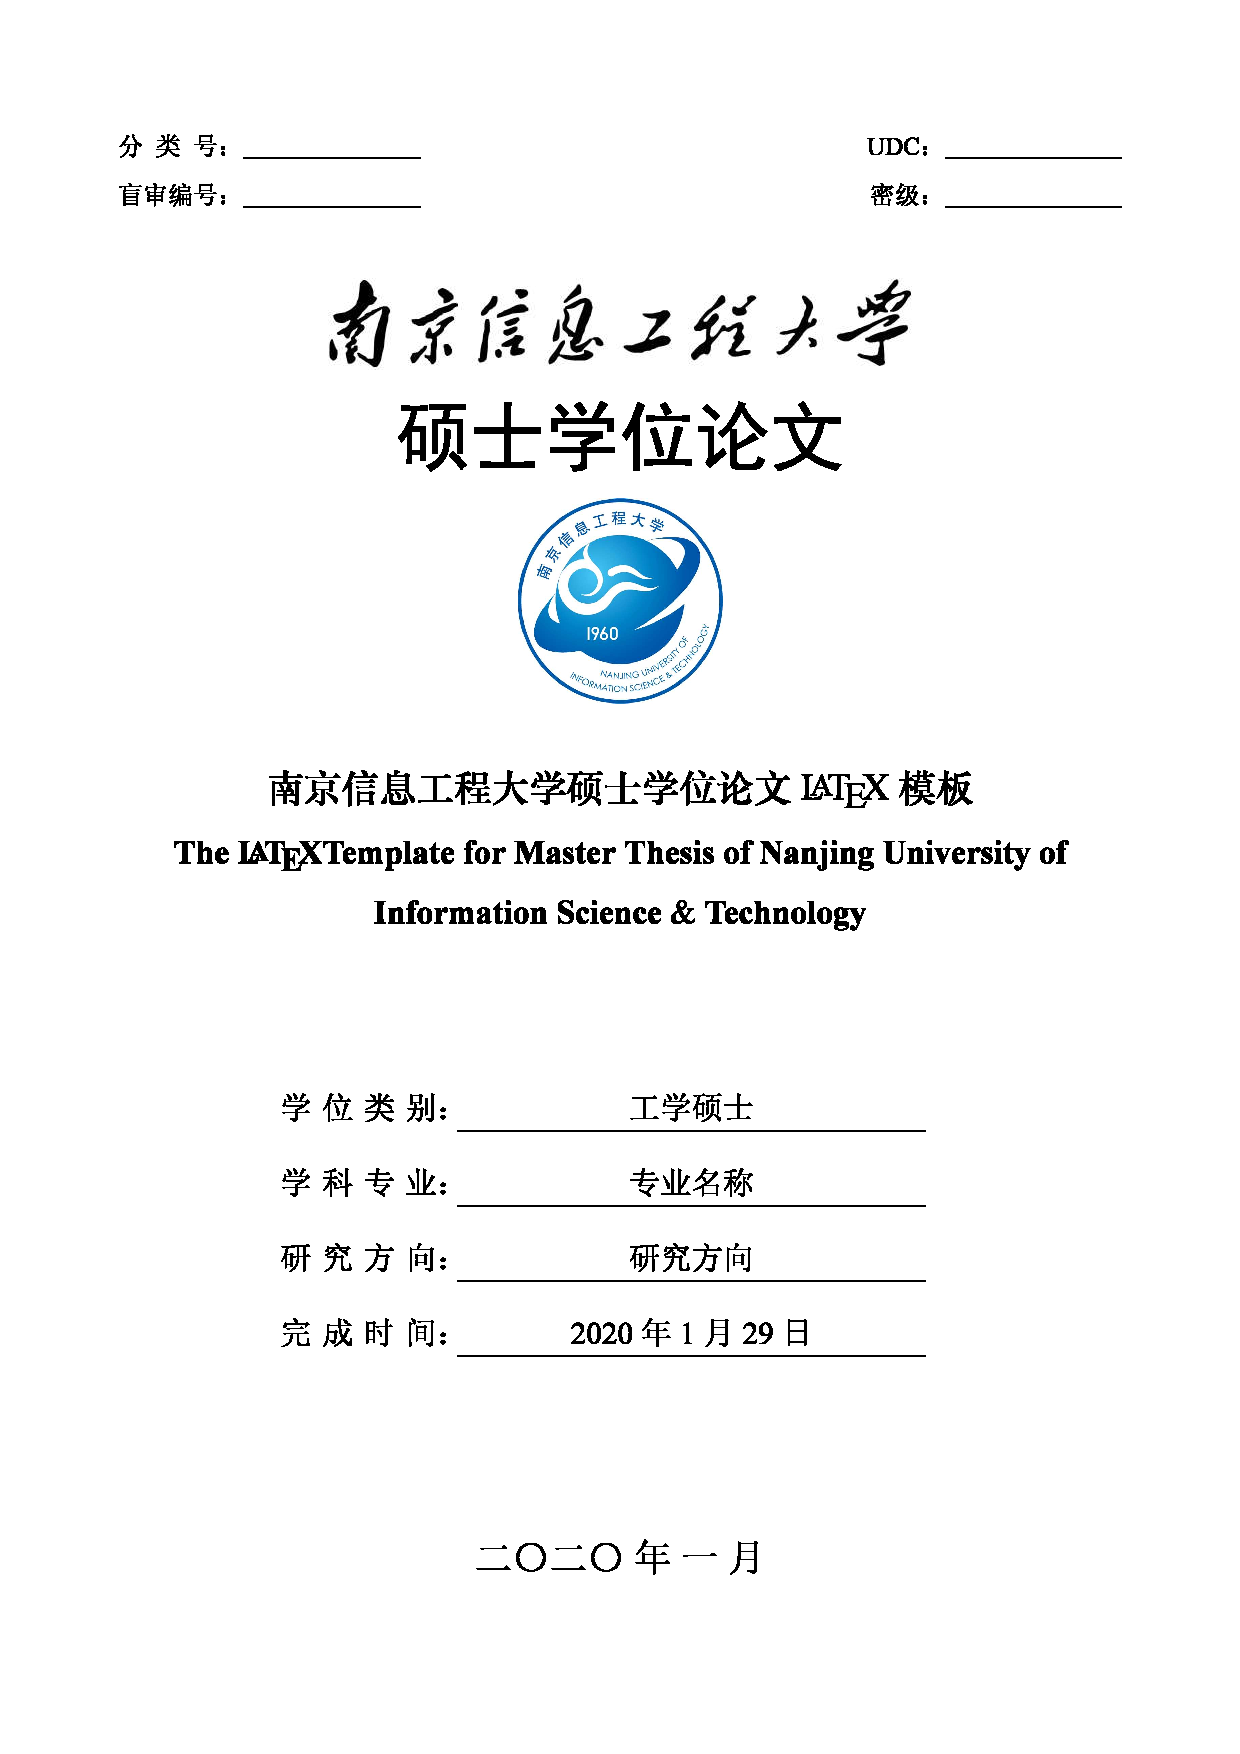
\includegraphics[width = 1\linewidth, keepaspectratio]{figs/blindtrial}
        \end{minipage}
    }
    \caption{两类封面示意图} \label{fig:title}
\end{figure}


\bibliographystyle{nuistbib}
\bibliography{sample}
\addreferencetoctl

\appendix

\chapter{}

本模板为方便个人硕士学位论文撰写所编写。由于本人对Tex编程不熟,大部分样式写法并不成熟,生搬硬套别人模板,未能自成一体。同时,本模板所提供的bib样式,修改自南京航空航天大学学位论文模板,感谢。模板若有问题,欢迎至\href{https://github.com/Alrash/NUIST_Master_Thesis}{GitHub仓库}提交Issue。

\backmatter

\chapter{致\quad{}谢}

本模板的编写,离不开以下几个开源项目的帮助,特此鸣谢!

\href{https://github.com/nuaatug/nuaathesis}{南京航空航天大学学位论文模板} 

\href{https://github.com/alwintsui/scutthesis}{华南理工大学学位论文Latex/Lyx模板} 

\href{https://gitee.com/MkSwQi/usstthesis}{上海理工大学本科毕业设计(论文) LaTeX 模板} 

\href{https://github.com/LirenW/NUIST_thesis_template_V2.0}{南京信息工程大学本科学位论文模板} 

\href{http://mirrors.ibiblio.org/CTAN/language/chinese/ctex/ctex.pdf}{CTEX宏集手册} 

\end{document}